\documentclass[tikz,border=8pt]{standalone}
% Shared TikZ style for synorg platform diagrams. Each diagram \input's this
% inside a standalone document. Palette tracks the Material "teal" site theme so
% figures read as one system in light mode (SVGs are theme-neutral otherwise).
\usetikzlibrary{arrows.meta,positioning,shapes.geometric,fit,backgrounds,calc,decorations.pathreplacing}

\definecolor{synteal}{HTML}{00897B}   % primary
\definecolor{synfill}{HTML}{E0F2F1}   % light fill
\definecolor{synamber}{HTML}{B26A00}  % warning / lend
\definecolor{synred}{HTML}{B00020}    % deny / danger
\definecolor{syngrey}{HTML}{5F6368}   % muted

\tikzset{
  >=Stealth,
  font=\sffamily\small,
  box/.style={draw=synteal,line width=0.6pt,rounded corners=2pt,fill=synfill,
              inner sep=5pt,align=center},
  plane/.style={draw=synteal,line width=0.8pt,rounded corners=3pt,fill=synfill,
                inner sep=8pt,align=center},
  state/.style={draw=synteal,line width=0.7pt,circle,fill=synfill,inner sep=3pt,
                minimum size=11mm,align=center,font=\sffamily\footnotesize},
  decision/.style={draw=synteal,line width=0.7pt,diamond,aspect=2,fill=synfill,
                   inner sep=1pt,align=center,font=\sffamily\footnotesize},
  deny/.style={draw=synred,fill=synred!8,text=synred},
  warn/.style={draw=synamber,fill=synamber!10},
  flow/.style={->,line width=0.6pt,draw=syngrey},
  flowlbl/.style={font=\sffamily\footnotesize,text=syngrey,inner sep=2pt},
  note/.style={font=\sffamily\footnotesize\itshape,text=syngrey},
}

\begin{document}
% Bootstrap order from zero (deploy-platform.md). The order is load-bearing:
% capacity is captured before anything can release it, and the game-day gate
% stands between the built platform and a live lending window.
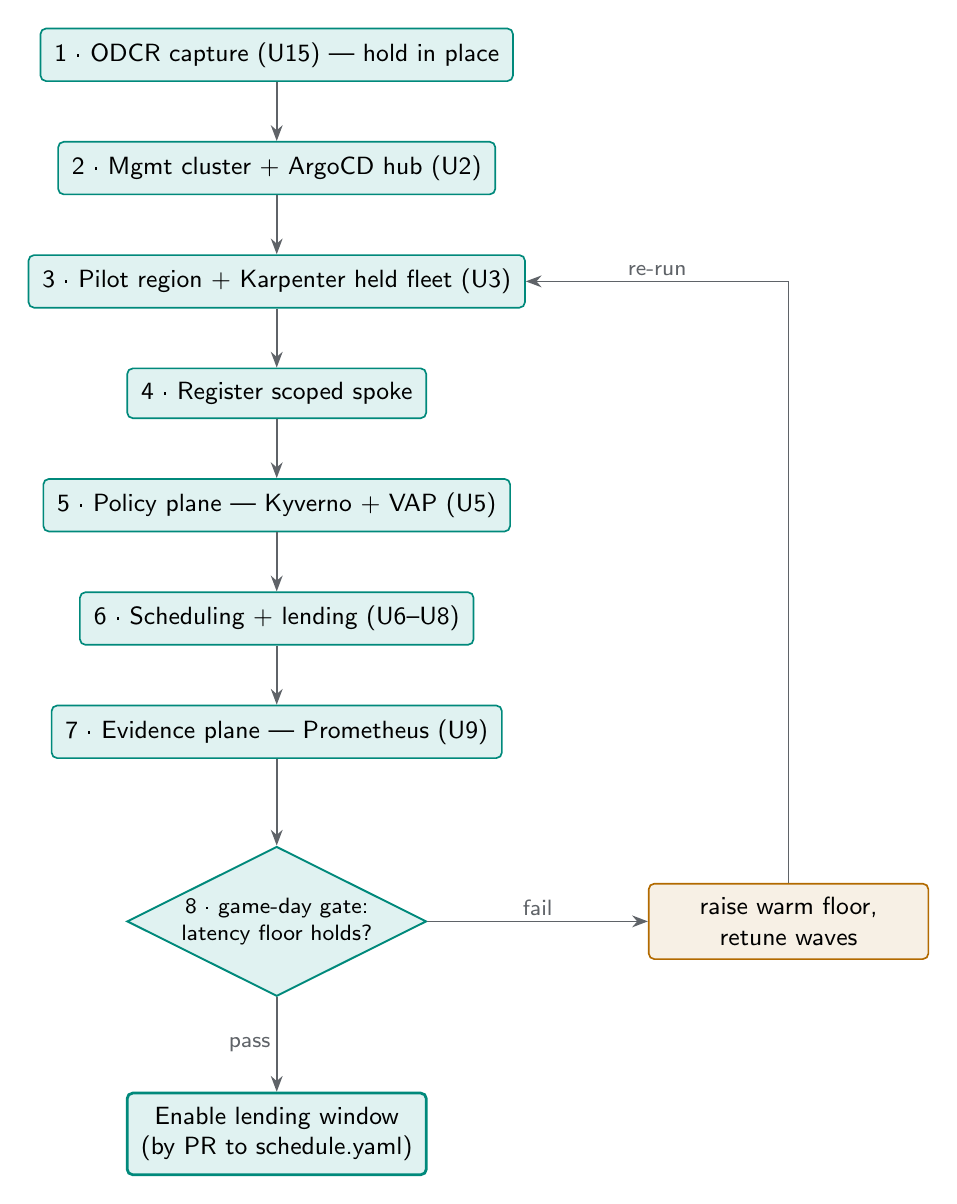
\begin{tikzpicture}[node distance=7.5mm]
  \node[box] (s1) {1 · ODCR capture (U15) --- hold in place};
  \node[box,below=of s1] (s2) {2 · Mgmt cluster + ArgoCD hub (U2)};
  \node[box,below=of s2] (s3) {3 · Pilot region + Karpenter held fleet (U3)};
  \node[box,below=of s3] (s4) {4 · Register scoped spoke};
  \node[box,below=of s4] (s5) {5 · Policy plane --- Kyverno + VAP (U5)};
  \node[box,below=of s5] (s6) {6 · Scheduling + lending (U6--U8)};
  \node[box,below=of s6] (s7) {7 · Evidence plane --- Prometheus (U9)};
  \node[decision,below=11mm of s7] (gd) {8 · game-day gate:\\latency floor holds?};
  \node[box,below=12mm of gd,line width=1pt] (enable)
    {Enable lending window\\(by PR to schedule.yaml)};
  \node[box,warn,right=28mm of gd,text width=32mm] (fix)
    {raise warm floor,\\retune waves};

  \draw[flow] (s1)--(s2); \draw[flow] (s2)--(s3); \draw[flow] (s3)--(s4);
  \draw[flow] (s4)--(s5); \draw[flow] (s5)--(s6); \draw[flow] (s6)--(s7);
  \draw[flow] (s7)--(gd);
  \draw[flow] (gd) -- node[flowlbl,left]{pass} (enable);
  \draw[flow] (gd) -- node[flowlbl,above]{fail} (fix);
  \draw[flow] (fix.north) |- node[flowlbl,near end,above]{re-run} (s3.east);
\end{tikzpicture}
\end{document}
